\section{Abstract}
	Millican's Oil Drop Experiment is used to determine the basic electric charge, or charge on an electron. We confirmed the quantization of charge in integer multiples of charge on an electron e in the experiment. The capacity to regulate, change, and balance extremely tiny forces of the order of 10-14 N is required for this experiment. In this experiment, small oil droplets from an atomizer are sprayed and allowed to fall between two plates, between which a potential difference may be used to provide force to the charged droplets owing to the electric field. The droplets become charged as they pass through the atomizer owing to frictional forces. Now, the droplet of appropriate size and charge is chosen and studied for forces under two conditions: The Dynamic method and Balancing method; to find their radii and charges.

\section{Experimental Setup}
	The experimental apparatus, as shown in the picture, comprises of an oil drop chamber with parallel plate electrodes at a 5mm spacing utilising a thick ebonite ring with a hole near the centre for seeing the droplets. A gadget lights the compartment, and a hole on the top plate permits droplets from the atomizer to enter. A CCD camera attached to a monitor may be used to see the droplets. The upper plate voltage may be regulated and measured with a voltage supply, while the lower plate is grounded. The free fall and rising times are calculated using a time metre.

	\begin{figure}[H]
		\centering
		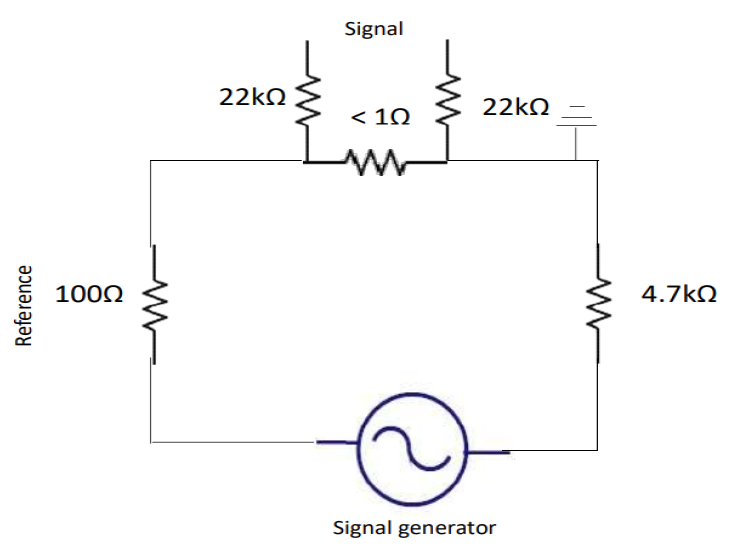
\includegraphics[width=0.5\textwidth]{2.png}
		\caption{Top View of the Panel}
		\label{fig:2}
	\end{figure}